\section{Implementation}
\label{sec:implementation}
We will have a look at the implementation of the engine and the framework in this section. Much focus lies on performance, and therefore, the

TODO: Diskusjonen kan derfor bli preget av hastighet osv.

\subsection{About Ngene}
\emph{Ngene} is a flexible, generic, multi-purpose genetic algorithm engine written in C++ with heavy emphasis on performance and flexibility. The engine is divided into logical modules that can be easily interchanged or extended upon in order to fit the intended goal. A sub-goal of this engine is also portability, as in the program should support any existing operating system and platform.

The prototype for this engine started out as an assignment for a sub-symbolic artificial intelligence course. It was written in Python, which later proved to be too slow for this kind of application, and later partially ported to C++ because I wanted to learn the language at the time. The project got lost in a pile of other assignments and was never heard from again. The engine was finally picked up again, and completed for the purpose of this thesis.

\subsubsection{Modular Design}
In order to achieve maximum flexibility, the engine should be able to change any of its parts without having to do anything special. Should the user feel like changing the mutation method, this should be as easy as changing a single line in a configuration file. More essentially, conducting experiments on different genotypes should also be just as easy as mentioned. With that in mind, the design is therefore broken into the following logical modules:

\begin{itemize}
	\itemsep=0pt
	\item\textbf{Core} - The genetic algorithm itself
	\item\textbf{Fitness} - Assesses the fitness of a genotype
	\item\textbf{Genotype} - Generates the genotype and translates them to phenotype
	\item\textbf{Mating} - Crosses two genotypes
	\item\textbf{Mutator} - Mutates a genotype
	\item\textbf{Selector} - Randomly selects a genotype
\end{itemize}

The engine is now like a jigsaw puzzle with pieces that resemble in shape but not motive. This way, it is possible to put together different pictures without having to perform any extraneous tasks (like cutting the edges to make it fit). More concretely, this modular design will allow users to swap a module, say roulette selection for tournament selection, without prior knowledge of programming. In fact, writing code will not at all be needed unless a new module is required. This design will also keep the code much cleaner and easier to maintain.

\subsubsection{Why C++?}
In a sense, one can say that this project was made possible because of my prototype in Python. It taught me many higher level concepts that is practically non-existant in lower level languages such as C++. Without it, I probably wouldn't have been able to bring the project to the level it is today. Especially without the concept of a dynamic type, the idea of a container that can contain anything from an integer, to a string, to a floating type number, I would still have trouble trying to compensate for it with complex algorithms to deal with raw data pointers. Most importantly, it taught me the importance of optimization and use of libraries.

Choosing a programming language depends on what kind of application you want to write. A simple program with no special requirements can be written in any language. For instance, a mail client written in Python will perform equally well as any other client because the focus lies on fetching and displaying e-mails and the ability to manage them in an easy way. The features are more important than the extra two milliseconds it takes to perform a query. However, there are applications for which performance is more important than anything. Arguably, such programs should be written in one of two ways: In assembly (or machine code) or C/C+. While assembly is rarely used these days due to being practically unreadable for mortals, C and C++ is often used for time critical applications. Unlike languages that depend on a virtual machine (C\#, Java), or an interpreter (some LISP dialects, Python), code written in C/C++ is compiled directly to machine code before executed, often yielding much better performance.

C++ is thought of as being a middle level language. It has the advantages of both the lower (machine code) and higher level languages, but also the inherent disadvantages. For example, all memory management must be explicitly handled in the code because C++ lacks a garbage collection found typically in C\# or Java. This means that we have to be careful of memory leaks and access of invalid memory addresses. Furthermore, C++ doesn't come with as big a convenience library as those found in aforementioned languages. Such a library would eliminate rewriting often used algorithms and the headache of fixing a buggy code. Fortunately, efforts are already being made to ease the implementation through external libraries.

\subsubsection{Boost C++ Libraries}
\emph{Boost}\footnote{\url{http://www.boost.org/}} is a collection of libraries which complement the C++ Standard Library (STL). Ngene makes use of this collection, saving time and effort, and guaranteeing that such code works as it should.

\paragraph{\textbf{Boost.Any}}\cite{henney2001}
A problem with writing a generic genetic algorithm in a strongly typed programming language, is that different studies require different data types to be passed around the system. CGP, for instance, uses integers to implement its genotype, while ArtDev3D uses a custom defined type. In other models, there may even be a mix of different types. It is impossible to foresee what may or may not be used, and we are thus forced to abstract this away. Unfortunately, C++ will not allow an integer variable to store any other data type than an integer. In a higher level language like Python, there exists a container that can store any type of data:

\begin{verbatim}
>>> foo = 1 + 2
>>> print foo
3
>>> foo = "awesome"
>>> print foo
awesome
>>> _
\end{verbatim}

This can also be done in C++ with some coding. Fortunately for us, this has already been implemented and is freely available as part of \emph{Boost}. The modular design would otherwise not work without it, at least not within given time constraint. The container, called \emph{Boost.Any}, does not differ much from the one found in Python and comes only at the cheap cost of requiring a type-casting before the data can be handled as normal.

\paragraph{\textbf{Boost Random Number Library}}\cite{maurer2000}
Another problem with genetic algorithms and development in general is implementing a good pseudo-random number generator. Ngene uses the implementation of \emph{Mersenne twister} pseudo-random number generator also found in the Boost libraries. This generator was chosen for its long period ($2^(19937) - 1$ to be exact), and because it is relatively fast compared to other algorithms. It also passes a number of tests for randomness, including Diehard\footnote{A collection of tests to measure the quality of the randomness of the generator, developed by George Marsaglia.} and most of the stricter TestU01 Crush\footnote{Another collection of tests, developed by Pierre L'Ecuyer and Richard Simard.} randomness tests.

\subsubsection{Brief System Overview}
\begin{figure}[!ht]
	\centering
	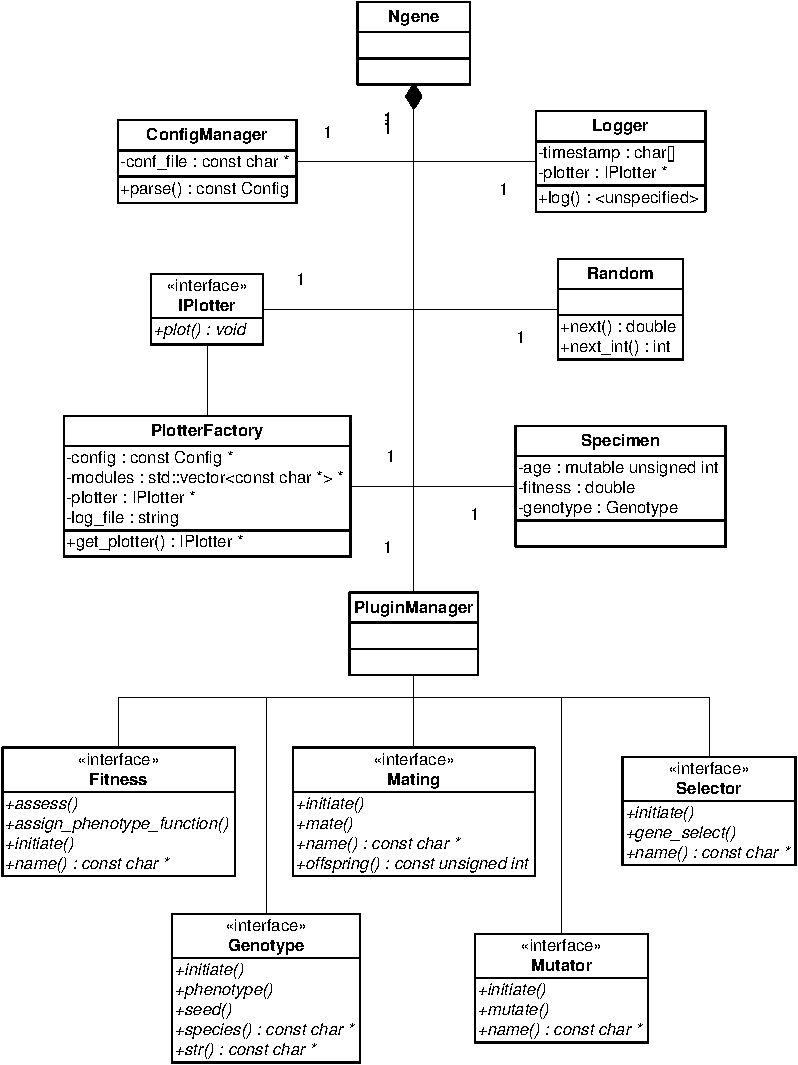
\includegraphics[scale=0.9]{diagram_ngene}
	\caption{Overview of Ngene}
	\label{fig:diagram_ngene}
\end{figure}

Figure~\ref{fig:diagram_ngene} shows a brief overview of how Ngene is put together. At startup, three of these parts are responsible for what must happen before anything can be run in accordance with the user's parameters. \texttt{ConfigManager} takes care of reading the configuration file and makes sure that all other parts have access to and will understand what it is told to do. Once it has played its part, \texttt{PluginManager} should be able to load relevant modules and \texttt{Logger} will know whether or not it should plot a fitness/generation graph of a population or just write some text to a file.

The genetic algorithm is very simple:
\begin{enumerate}
	\itemsep=0pt
	\item An initial population is randomly generated.
	\item \texttt{Specimen}s are randomly selected for crossover.
	\item Repeat step 2 until the offspring population is of satisfactory size.
	\item Replace adult population with offspring population.
	\item Repeat process from step 2 until the maximum number of generations is reached, or a perfect \texttt{Specimen} is found.
	\item Write log/graph and final \texttt{Specimen} to disk.
\end{enumerate}

The final step is the responsibility of \texttt{Logger}. \texttt{Logger} has no knowledge of what format the \texttt{Specimen} should be written as. Be it a text file, an image or a proprietary format, it will simply request the \texttt{Genotype} module to give it some data to write to disk. The output format is actually hard-coded into each \texttt{Genotype} module. Because this rarely changes for a single experiment and/or model, otherwise a new module must be written anyway, this has no real impact on users.

\texttt{PluginManager}, along with the responsibilities of loading and releasing modules, will also act as a layer between the modules and the algorithm itself. The engine will never have to bother with the specifics of each module, but rather be able to just tell what a module ought to do. Of course, this requires that the modules follow certain specifications in order to be compatible with this layer. These are described in more detail in the system documentation for Ngene.


\subsection{Ngene Development Framework}
\begin{figure}[!ht]
	\centering
	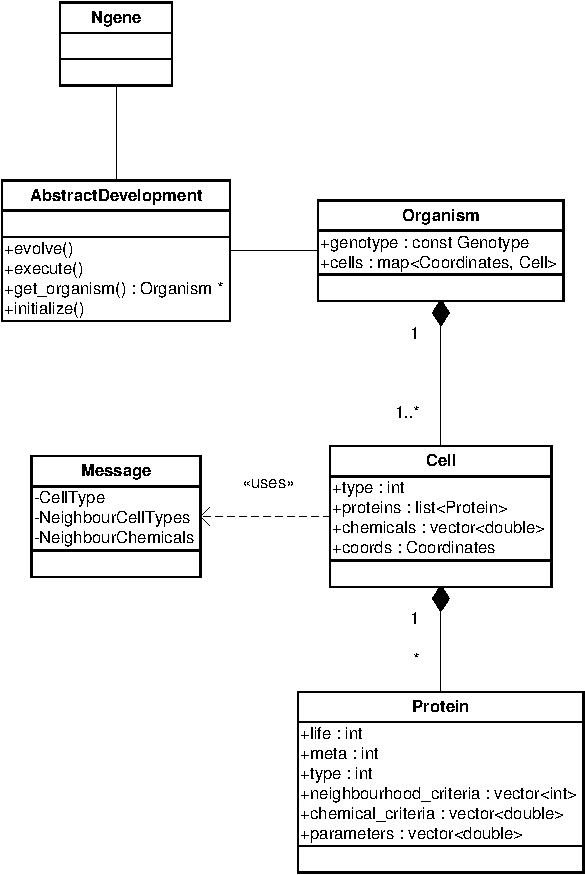
\includegraphics[scale=0.9]{diagram_ndevframe}
	\caption{Overview of Ngene Development Framework}
	\label{fig:diagram_ndevframe}
\end{figure}

As it stood, Ngene gave the users too much freedom in implementing their own modules, making it difficult to compare two models without having to factor in differences in implementations. A generic development framework was therefore devised to eliminate these factors and ease the implementation at the same time. The framework was designed to accommodate any conceivable model.

The framework provides a code base that implements a common development algorithms, along with common concepts such as a cell or a protein (see fig.~\ref{fig:diagram_ndevframe}). This includes intercellular communication (see fig.~\ref{fig:diagram_ndevframe_msg}) and development stepping in order to reduce any implementation advantages a model has over another. Use of this code base is enforced in order to ensure that all comparison made between different development models will be based on a common ground.

\begin{figure}[!ht]
	\centering
	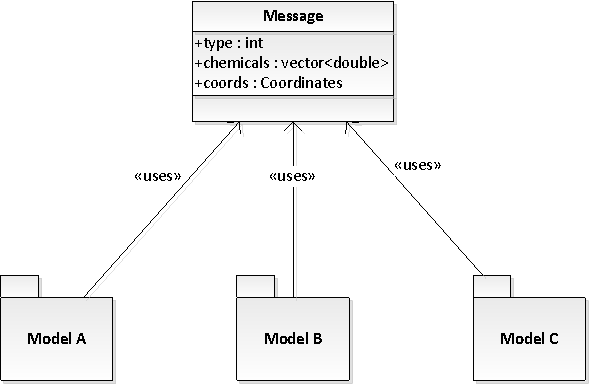
\includegraphics[scale=0.9]{diagram_ndevframe_msg}
	\caption{A common message implementation should eliminate factors involving what information is exchanged between the organism's cells.}
	\label{fig:diagram_ndevframe_msg}
\end{figure}

Figure~\ref{fig:diagram_ndevframe_common-base} shows three different scenarios where model A and B use only chemicals, while model C only makes use of proteins. This tells us that model A and B may use both the cell type and the chemicals part of a \texttt{Message}, while model C only takes cell type into consideration (or it may not even make use of communication). We also see that model B and C make use of a control program besides the genome. Even though these three models are different, they still use the same framework or code base. A comparison can then be performed without having to take into account implementation differences that may affect one model or another.

\begin{figure}[!ht]
	\centering
	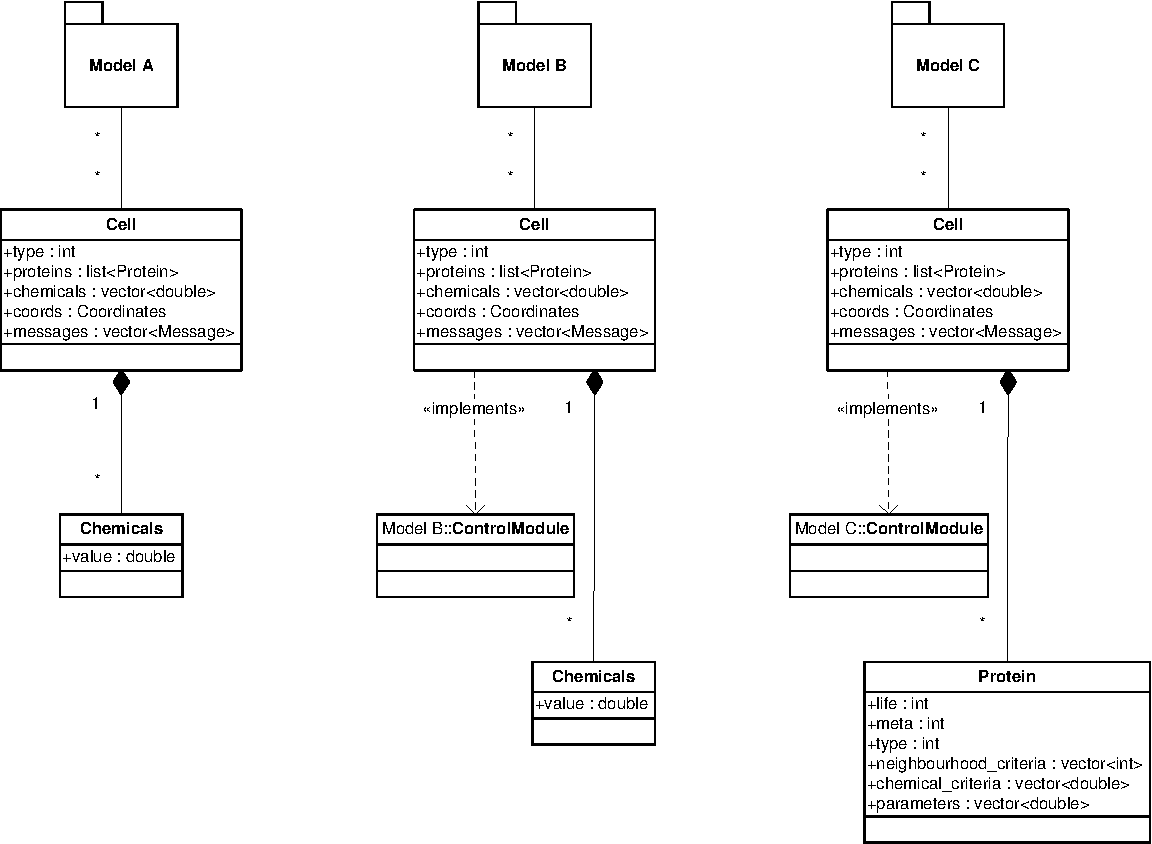
\includegraphics[scale=0.8]{diagram_ndevframe_common-base}
	\caption{Albeit different, all three models still use the same implementation of a cell, chemicals and proteins, and receive the same messages.}
	\label{fig:diagram_ndevframe_common-base}
\end{figure}

With regards to speed optimizations, lots of thought as been put into how to represent the organisms themselves. In the current implementation, a C++ Standard Library (STL) \texttt{<map>} is used to store the cells using their coordinates as the key value. Other alternatives were also considered:

\begin{center}
	\begin{tabular}{ r | c | c | c }
		~ & STL \texttt{<map>} & STL \texttt{<vector>} & STL \texttt{<ext/hash\_map>} \\
		\hline
		element access & $O(log~n)$ & $O(1)$ & $O(1)$ \\
		\hline
		insertion & $O(log~n)$ & $O(1)$ & $O(1)$ \\
		\hline
		search & $O(log~n)$ & $O(n)$ & $O(1)$ \\
	\end{tabular}
	\label{tbl:speed}
\end{center}

A quick glance at the comparison table and the \texttt{<ext/hash\_map>} may seem like the best choice to go with. However, there are some drawbacks that must be taken into consideration. A good hashing algorithm is essential for the performance of the hash table by providing a uniform distribution over the array. Too simple, and a lot of collisions will occur, but too complex and the hashing table will spend all of its time calculating a hash value. Collisions occur regardless of how good the algorithm is. The \emph{birthday paradox} predicts that it doesn't take many elements before the chance of a collision exceeds 95\%, even for very big arrays. A good collision resolution is therefore also needed but will not be enough to guarantee the performance advantage over other solutions. For the experiments conducted in this thesis, the number of cells rarely exceeded 1000. For a \texttt{<map>}, this means at most 10 comparisons is needed to find an element by its key value. A hash table would require about the same number of operations to calculate the hash, perform the lookup and resolve any collisions.

The \texttt{<map>} was chosen over the \texttt{<vector>} because despite its better access and insertion times, required more time to find all of a cell's neighbours. This can be remedied by creating and maintaining a neighbours list for every cell. However, this would make insertion $O(n)$ as opposed to $O(log~n)$ of the \texttt{<map>}.

\subsubsection{Using the Framework}
\begin{figure}[!ht]
	\centering
	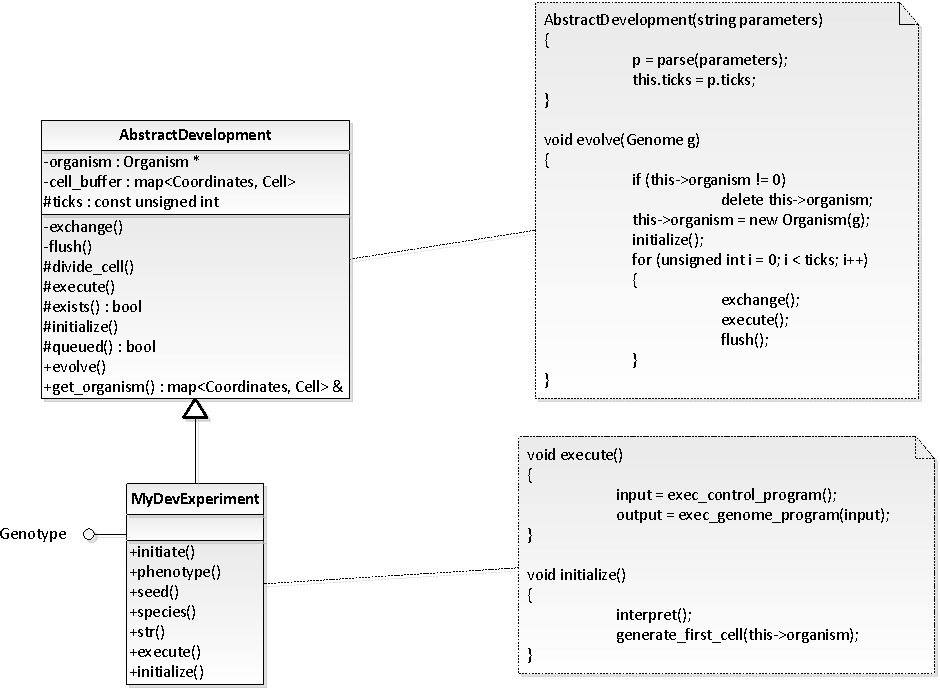
\includegraphics[scale=0.9]{diagram_ndevframe_ex}
	\caption{An example of how one can implement \texttt{MyDevExperiment}.}
	\label{fig:diagram_ndevframe_ex}
\end{figure}

The framework was designed to ease the implementation effort as much as possible. The whole code base can be inherited from \texttt{AbstractDevelopment} (see fig.~\ref{fig:diagram_ndevframe_ex}). To port a model to this framework, only two functions need to be implemented: \texttt{execute()} and \texttt{initialize()}. The latter is executed once with every new organism that is to be developed, and can be used to unpacking the genotype to a cellular program and/or generating initial cells in the organism. The \texttt{execute()} function is called every development step/tick, for every cell in the organism. Here, the cell program from the genotype can be executed as well as any control programs that might be needed. Note that any messages sent has already been received and are stored in the cells themselves by the time a cell is given the chance to fulfil its purpose in a tick. It will not be possible to actually access the organism itself from this function in order to avoid accidental tampering.

For the purpose of this thesis, two models were implemented within this framework not only to test the flexibility and performance of this framework but also to see what is missing and what areas need improvement.

\subsubsection{ArtDev3D}
Porting Johan H{\o}ye's master's thesis\cite{hoye2006} to Ngene's framework has been a matter of finding out what occurs in a cell during a development step, and whether or not there are external processes that needs to be accounted for. As described in \ref{sec:ArtDev3D}, the genotype of the model does not do all the work in a cell. The cell has its own control program as well. The program can be summarized as the following steps:

\begin{enumerate}
	\itemsep=0pt
	\item Clear all queued actions.
	\item For every active protein, queue their action requests.
	\item Accumulate actions (add them together to execute in one go).
	\item Execute action \#1: Transcribe proteins.
	\item Execute action \#2: Regulate chemical levels.
	\item Execute action \#3: Perform cell division.
	\item Execute action \#4: Change cell type.
	\item Remove dead proteins.
\end{enumerate}

The implementation of the model might seem overwhelming at first impression. There is a heavy use of biological concepts in the code and the simplest operation may span across many classes, and files, as a result. This alone makes it hard to follow the code flow, but the little system documentation that does exist, fortunately, does provide with some help though it consists mainly of commentaries in the source files themselves. While his efforts in making it understandable are much appreciated, it might be beneficial to flatten the structure a bit and get rid of some of the redundant structures that are inspired by nature. There is another reason for why this was altered as well.

In theory, such an implementation can have a negative impact on performance. When a simple operation performed must call a function to call another function to call yet another function and so on, can put the calling stack under strain. This may occur because this does not happen only once, but several times every development step in a single cell. And as we know, there are plenty of cells in an organism. Flattening the structure as mentioned, will reduce the number of calls and potentially improve performance.

There was also an issue that was identified and patched in the port. In most models, cells are developed simultaneously. In order to achieve this, information must be exchanged between all cells before a cell can execute its functions. This is to ensure that the cell program will execute based on the current state of the organism without interfering for other cells. In ArtDev3D, this is not properly implemented. Upon execution, the cell will start collecting requests from its proteins. The proteins can request an action when they are activated, i.e. when the state of the cell and its neighbours are above a threshold. The requests are queued up and then executed. The problem with this, is that it all happens in a single step. Thus, cells that already have had their turn before the current cell, will have an altered state. Actions are therefore based on a mix of ``newer'' information from these cells, and ``old'' information from the rest. When porting this code to the new framework, the cell will no longer have direct access to other cells. Instead, it will receive messages from (or a snapshot of) nearby cells before the development step takes place in any cell. This change may alter the outcome of the model, but was addressed merely out of necessity. We cannot have two different development algorithms as that would defeat the very purpose of the framework.


\subsubsection{Cartesian}
This model is based on a number of works by Julian F. Miller, mainly \cite{mteurogp2000} and \cite{ecal2003}.

TODO

Mutation upwards has an impact
Implement bit check error

\subsubsection{Performance}
So far, we've discussed the potential performance gain of this framework without actually seeing any gains.

TODO

